\documentclass[border=6pt,tikz]{standalone}
\usepackage{tikz}
\usepackage{amsmath,amssymb}
\usetikzlibrary{arrows.meta,positioning,fit,backgrounds,calc,shapes.geometric,decorations.pathreplacing,patterns}
\definecolor{ink}{HTML}{1B2430}
\definecolor{muted}{HTML}{6B7785}
\definecolor{accent}{HTML}{2F6FB5}
\definecolor{accent2}{HTML}{C1611F}
\definecolor{good}{HTML}{2E7D5B}
\definecolor{soft}{HTML}{EDF2F7}
\definecolor{soft2}{HTML}{FBEDE2}
\definecolor{soft3}{HTML}{E6F0E9}
\tikzset{
  box/.style={draw=ink,line width=.7pt,rounded corners=2pt,fill=soft,inner sep=4pt,align=center,font=\sffamily\small},
  boxa/.style={box,fill=soft2},
  boxb/.style={box,fill=soft3},
  plain/.style={align=center,font=\sffamily\small,text=ink},
  tiny/.style={align=center,font=\sffamily\scriptsize,text=muted},
  ar/.style={-{Stealth[length=2.4mm]},draw=ink,line width=.7pt},
  arm/.style={-{Stealth[length=2.4mm]},draw=muted,line width=.6pt,dashed},
  nd/.style={circle,draw=ink,line width=.7pt,fill=white,minimum size=7mm,inner sep=0pt,font=\sffamily\scriptsize},
  ndf/.style={nd,fill=soft},
  ndt/.style={nd,fill=soft2},
}

\begin{document}
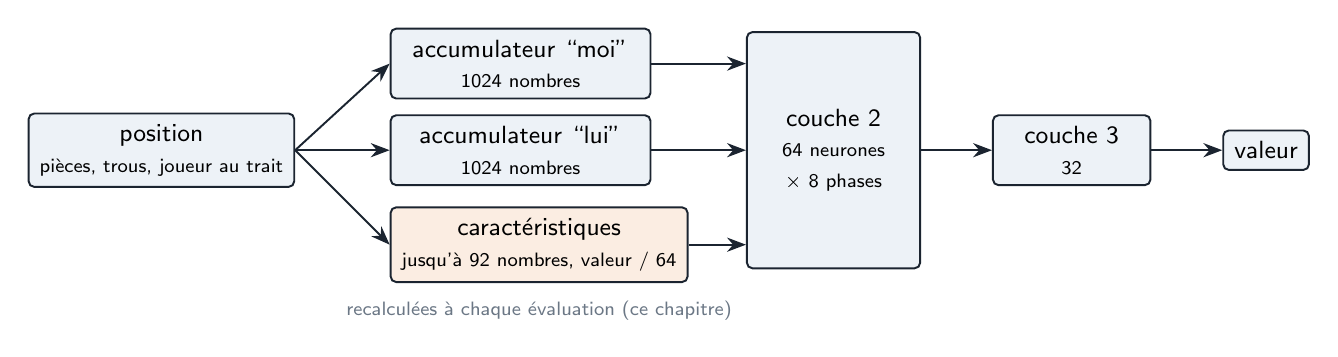
\begin{tikzpicture}[node distance=6mm and 9mm]
  \node[box,minimum width=27mm] (pos) {position\\\scriptsize pièces, trous, joueur au trait};
  \node[box,right=12mm of pos,yshift=11mm,minimum width=33mm] (us) {accumulateur ``moi''\\\scriptsize 1024 nombres};
  \node[box,right=12mm of pos,minimum width=33mm] (them) {accumulateur ``lui''\\\scriptsize 1024 nombres};
  \node[boxa,right=12mm of pos,yshift=-12mm,minimum width=33mm] (feat) {caractéristiques\\\scriptsize jusqu'à 92 nombres, valeur / 64};
  \node[box,right=12mm of them,minimum height=30mm,minimum width=22mm] (fc2) {couche 2\\\scriptsize 64 neurones\\\scriptsize × 8 phases};
  \node[box,right=9mm of fc2,minimum width=20mm] (rest) {couche 3\\\scriptsize 32};
  \node[box,right=9mm of rest] (v) {valeur};
  \draw[ar] (pos.east) -- (us.west);
  \draw[ar] (pos.east) -- (them.west);
  \draw[ar] (pos.east) -- (feat.west);
  \draw[ar] (us.east) -- (fc2.west |- us.east);
  \draw[ar] (them.east) -- (fc2.west |- them.east);
  \draw[ar] (feat.east) -- (fc2.west |- feat.east);
  \draw[ar] (fc2) -- (rest);
  \draw[ar] (rest) -- (v);
  \node[tiny,below=1mm of feat] {recalculées à chaque évaluation (ce chapitre)};
\end{tikzpicture}
\end{document}
